\chapter{Resultado final}\label{sec:final}
En esta sección se muestra el producto desarrollado, explicando en que consiste el juego y las decisiones con respecto al diseño que se han tomado. Todo el código del proyecto se puede encontrar en~\cite{bib:repositorio}, repositorio alojado en GitHub. La estructura del proyecto se puede consultar en el Apéndice~\ref{ap:estructura}. Además, en el repositorio se proporciona una versión del juego ya preparada para su prueba en emuladores o en hardware. Este archivo, junto al código de esa versión, se puede encontrar en la sección de ``Releases'' del repositorio. Un ejemplo de una versión publicada del juego se puede observar en la Figura~\ref{fig:release}.

\begin{figure}[h]
	\centering
	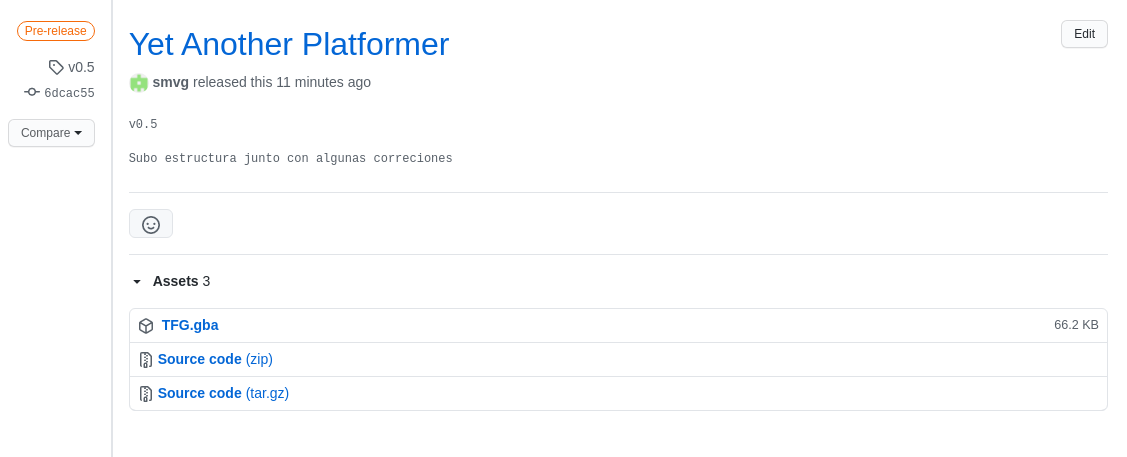
\includegraphics[width=.8\textwidth]{capitulos/capitulo6/release.png}
	\caption{Versión publicada del juego.}\label{fig:release}
\end{figure}
\FloatBarrier{}

\section{\textit{YAP} - \textit{Yet Another Platformer}}

\begin{figure}[b]
	\centering
	
\includegraphics[width=.5\textwidth]{capitulos/capitulo6/logo.png}
	\caption{Logo del juego \textit{Yet Another Platformer}.}\label{fig:logo}
\end{figure}

El juego, titulado \textit{YAP} (\textit{Yet Another Platformer}, logo en la Figura~\ref{fig:logo}), pone al jugador en el lugar de un mago que tiene que progresar por cada nivel, derrotando a los enemigos que encuentre por el camino. Los controles utilizados para moverse por el mapa son los habituales para juegos de este género, el botón izquierdo para moverse a la izquierda y el botón derecho para moverse a la derecha.

El mago que controla el jugador deberá alternar entre dos formas distintas, la azul y dorada, para poder progresar en el juego. Esto se debe a que cada una de las variantes tiene habilidades imprescindibles para completar cada uno de los niveles:

\begin{itemize}
	\item Variante azul: La variante azul, la cual se activa pulsando el botón ``L'', permite al jugador moverse con más rapidez con tal de poder escapar con facilidad de los enemigos. Además permite al jugador saltar a las estructuras elevadas que encontrará en cada uno de los niveles presionando el botón ``A''. La limitación de esta variante aparece al enfrentarse con los enemigos ya que no puede atacar, para ello el jugador tendrá que transformarse en la variante dorada del mago.
	\item Variante dorada: La variante dorada, la cual se activa pulsando el botón ``R'', limita el movimiento del jugador, ralentizando su velocidad en el eje X e imposibilitando su movimiento en el eje Y. Sin embargo, ahora el jugador tiene la posibilidad de atacar a los enemigos que se encuentren en proximidad presionando el botón ``B''.
\end{itemize}

\section{Personajes}

Los personajes del juego, excepto por algunas modificaciones menores, son todos obra de \textit{\href{https://o-lobster.itch.io/}{o\_lobster}}. La primera versión del juego cuenta con el mago mostrado en el \textit{spritesheet} de la Figura~\ref{fig:hero}. En la primera fila se observan las imágenes utilizadas para cuando el personaje no se mueve. La segunda fila muestra las imágenes utilizadas para cuando el personaje se mueve por tierra. En la tercera y cuarta fila se observan las imágenes para cuando el personaje cae de una posición elevada y salta. En la quinta y sexta fila se observan las imágenes utilizadas para animar el ataque del personaje, siendo la quinta fila la correspondiente al personaje y la sexta la correspondiente a la espada que saca el mismo. Por último, la última fila, muestra las imágenes utilizadas para la animación de la muerte del personaje. Para separar la animación de muerte de las demás, se ha optado también por parar de actualizar todas las demás animaciones cuando se de el caso (dejando al personaje como la única entidad animada). Cada una de los estados que puede tener el personaje (inactivo, corriendo, saltando y atacando), se actualiza la animación cada 10 fotogramas. Este comportamiento también se observa para los enemigos. En caso de agotar las imágenes destinadas a un estado en particular, se vuelve a empezar por la primera imagen. Un estado que no se incluye en el \textit{spritesheet} es el estado cuando el personaje es atacado. Tomando como inspiración algunos juegos de la época, se ha optado por hacer que el \textit{sprite} parpadeé para señalar que ha recibido daño de un enemigo para así rebajar el número de \textit{tiles} utilizados. Este efecto se consigue activando y desactivando el \textit{sprite} cada cierto periodo de tiempo.

\begin{figure}[h]
	\centering
	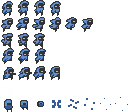
\includegraphics[height=5cm]{capitulos/capitulo6/hero.png}
	\caption{Los \textit{sprites} del personaje principal.}\label{fig:hero}
\end{figure}
\FloatBarrier{}

La variante dorada del personaje utiliza exactamente el mismo \textit{spritesheet} de la Figura~\ref{fig:hero} pero especificando una paleta de colores alterna. La transición entre cada uno de los estados hace uso del efecto mosaico para así dar la sensación que el mago se está transformando. La Figura~\ref{fig:hero_variants} muestra a los dos personajes.


\begin{figure}[h]
	\centering
	\begin{subfigure}[b]{0.45\textwidth}
		\centering
		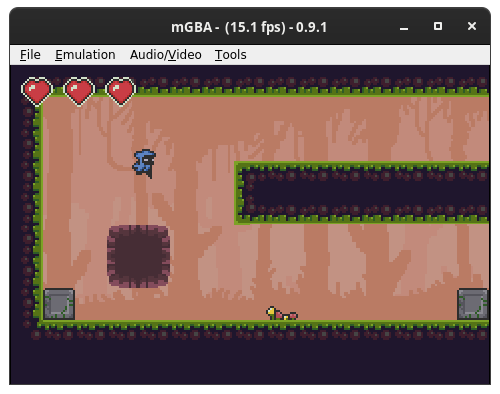
\includegraphics[width=\textwidth]{capitulos/capitulo6/hero_blue.png}
		\label{fig:hero_blue}
		\caption{Variante azul saltando.}
	\end{subfigure}
	\hfill
	\begin{subfigure}[b]{0.45\textwidth}
		\centering
		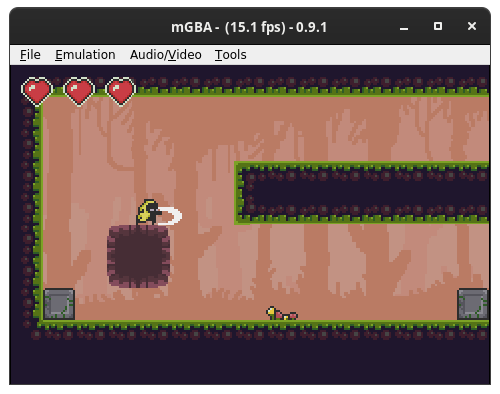
\includegraphics[width=\textwidth]{capitulos/capitulo6/hero_gold.png}
		\label{fig:hero_gold}
		\caption{Variante dorada atacando.}
	\end{subfigure}
	\caption{Las dos variantes del personaje principal.}
	\label{fig:hero_variants}
\end{figure}
\FloatBarrier{}

Los dos enemigos incluidos en el juego cuentan con animaciones y estados más simples que el personaje principal. El primer enemigo, el ``monstruo verde'' cuenta con dos estados, el estado en movimiento o inactivo, y el estado de muerte del enemigo. El \textit{spritesheet} se puede observar en la Figura~\ref{fig:slime}. Este enemigo se mueve de forma independiente hasta detectar una colisión en el eje X o vacío en el eje Y (una caída). Cuando detecta la colisión invertirá su posición.

\begin{figure}[h]
	\centering
	
\includegraphics[height=2cm]{capitulos/capitulo6/slime.png}
	\caption{Los \textit{sprites} del primer enemigo.}\label{fig:slime}
\end{figure}

El otro enemigo, la ``mosca'', al igual que el ``monstruo verde'', cuenta con dos estados, el estado en movimiento o inactivo, y el estado de muerte del mismo. El \textit{spritesheet} se puede observar en la Figura~\ref{fig:fly}. A diferencia del ``monstruo verde'', este enemigo puede moverse sin tener ningún bloque sólido por debajo, aunque si se encuentra de frente con un bloque invertirá su orientación.

\begin{figure}[h]
	\centering
	
\includegraphics[height=2cm]{capitulos/capitulo6/fly.png}
	\caption{Los \textit{sprites} del segundo enemigo.}\label{fig:fly}
\end{figure}

Los dos enemigos renderizados en un nivel se pueden observar en la Figura~\ref{fig:enemies}. Para una demostración más extensiva de los diferentes estados de cada personaje consultar el Apéndice~\ref{ap:personajes}.

\begin{figure}[h]
	\centering
	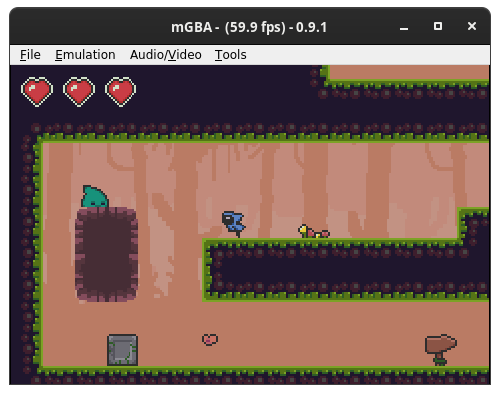
\includegraphics[width=.7\textwidth]{capitulos/capitulo6/enemies.png}
	\caption{Enemigos de uno de los niveles.}\label{fig:enemies}
\end{figure}

\section{\textit{Title screens}, menús y niveles}
Cada uno de los créditos, menús y niveles reciben el nombre de ``escenas'' en el código, término que se utiliza en motores gráficos como Unity. Los créditos iniciales del juego muestran el logo de la Universidad de Almería (aprovechando los fondos \textit{bitmap} del dispositivo) y todas las personas cuyos recursos han sido utilizados. Dos ejemplos, incluyendo el logo y el nombre del autor se pueden observar en la Figura~\ref{fig:credits}. Para el resto de escenas consultar el Apéndice~\ref{ap:escenas}.

La siguiente escena con la que el jugador se encuentra, una vez acabados los créditos iniciales del juego, es el menú principal. El menú principal cuenta con fondos y \textit{sprites} animados y una imagen proveniente del emulador se puede observar en la Figura~\ref{fig:menu}. Las diferencias observadas entre el menú actual y los mostrados previamente se deben a cambios durante el desarrollo del juego. El menú definitivo es el mostrado en la Figura~\ref{fig:menu}.

\begin{figure}[h]
	\centering
	\begin{subfigure}[b]{0.45\textwidth}
		\centering
		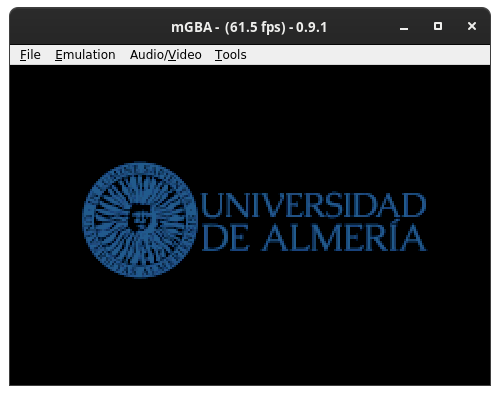
\includegraphics[width=\textwidth]{capitulos/capitulo5/game_0.png}
		\label{fig:credit_logo}
		\caption{\textit{Title screen} con el logo de la UAL.}
	\end{subfigure}
	\hfill
	\begin{subfigure}[b]{0.45\textwidth}
		\centering
		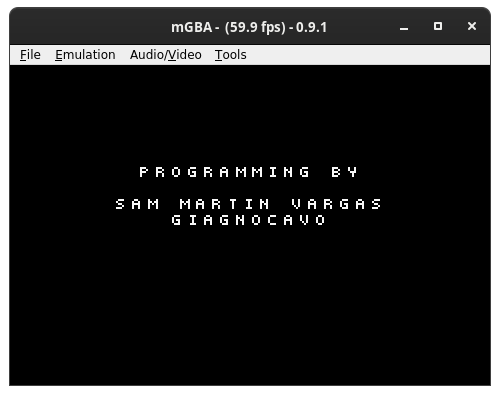
\includegraphics[width=\textwidth]{capitulos/capitulo5/game_1.png}
		\label{fig:credit_nombre}
		\caption{Game Boy Advance Micro}
	\end{subfigure}
	\caption{\textit{Title screen}.}
	\label{fig:credits}
\end{figure}
\FloatBarrier{}

\begin{figure}[h]
	\centering
	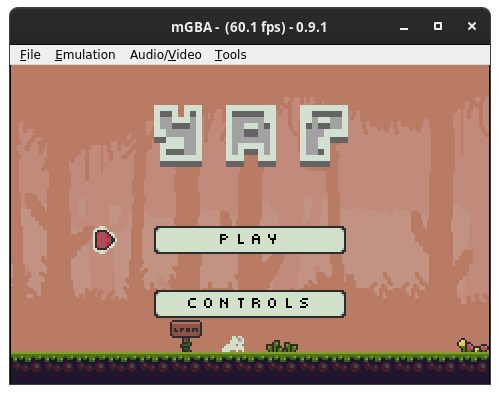
\includegraphics[width=.6\textwidth]{capitulos/capitulo6/menu.png}
	\caption{Menú principal del juego.}\label{fig:menu}
\end{figure}
\FloatBarrier{}

Aquí el jugador puede empezar una partida, o seguir el progreso en caso de haber jugador anteriormente, y consultar los controles del juego. En la escena de controles, se incluye un espacio para que el jugador pueda probarlos tal y como se puede observar en la Figura~\ref{fig:controls}.

\begin{figure}[h]
	\centering
	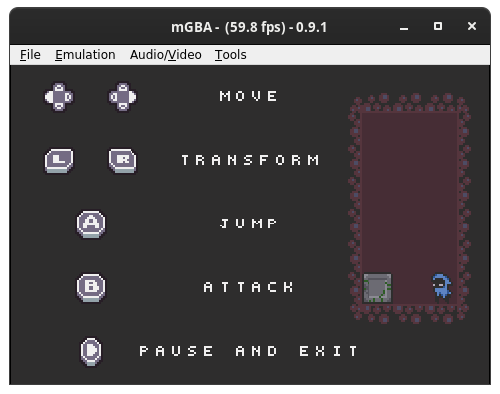
\includegraphics[width=.6\textwidth]{capitulos/capitulo6/controls.png}
	\caption{Escena de controles del juego.}\label{fig:controls}
\end{figure}
\FloatBarrier{}

El primer nivel del juego cuenta con pequeñas indicaciones para guiar al jugador durante su primera partida. Las dos escenas que conforman el primer nivel se pueden apreciar en la Figuras~\ref{fig:lvl1_0} y~\ref{fig:lvl1_1}. A pesar de no forzar al jugador a realizar las indicaciones mostradas, el diseño del primer nivel requiere que el jugador sepa realizar todas las acciones y funcionalidades para poder completarlo. El resto de niveles se puede observar en el Apéndice~\ref{ap:escenas}.

\vspace{1cm}

\begin{figure}[h]
	\centering
	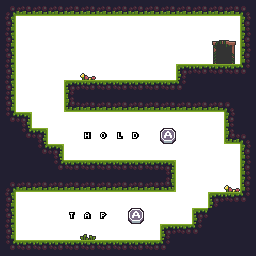
\includegraphics[width=.55\textwidth]{capitulos/capitulo6/level_1_0.png}
	\caption{Primera parte del nivel.}\label{fig:lvl1_0}
\end{figure}

\begin{figure}[h]
	\centering
	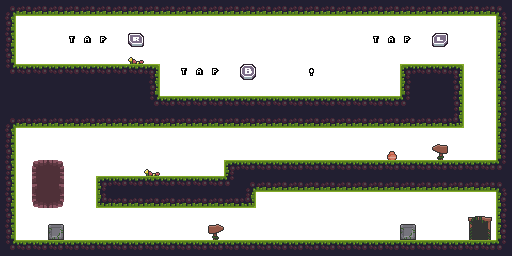
\includegraphics[width=.9\textwidth]{capitulos/capitulo6/level_1_1.png}
	\caption{Segunda parte del nivel.}\label{fig:lvl1_1}
\end{figure}
\FloatBarrier{}

Todos los niveles del juego utilizan los 4 fondos ``normales'' que ofrece la GBA. El primero de ellos se reserva para cualquier estructura que provoque una colisión con el personaje y enemigos, el suelo por ejemplo. El segundo fondo se utiliza para aquellos objetos que forman parte del nivel pero no provocan colisiones. El tercer fondo, se reserva para el fondo naranja utilizado en la Figura~\ref{fig:menu}. Finalmente, el cuarto fondo se utiliza para guardar el menú in-game, el cual solo se activa si el jugador presionar ``Start''. 

\section{Música}
Dado que no se puede demostrar las dos piezas de música utilizadas para el juego, realizadas por \textit{\href{https://gooseninja.itch.io/}{Goose Ninja}}, se comentará brevemente la implementación por \textit{Direct Sound}.

En el juego, se hacen uso de dos muestras de audio, diseñadas para poder reproducirse en ciclo sin cortes. Para hacer posible su reproducción en el dispositivo, se han convertido a una frecuencia de 16 KHz a 8 bits. Cada ciclo se realiza a partir de los contadores del dispositivo y de las transferencias \textit{DMA} de tipo 1. Las transferencias además se configuran para que ocurran cada vez que el buffer de audio se quede vacío.

\section{Indicadores in-game}
El único indicador utilizado es el número de corazones (vida) con el que cuenta el personaje. El indicador se localiza en la esquina superior izquierda, y al aparecer el personaje realiza una pequeña animación para llamar la atención del jugador. A diferencia del resto animaciones, esta depende de la matriz de transformación ya que cambia la escala de un tamaño inapreciable al tamaño original en un corto periodo de tiempo. En la Figura~\ref{fig:heart} se pueden observar el estado inicial y final de la animación. Dado que los corazones denotan la vida del jugador, estos irán desapareciendo conforme el jugador pierde vida.

\begin{figure}[h]
	\centering
	\begin{subfigure}[b]{0.45\textwidth}
		\centering
		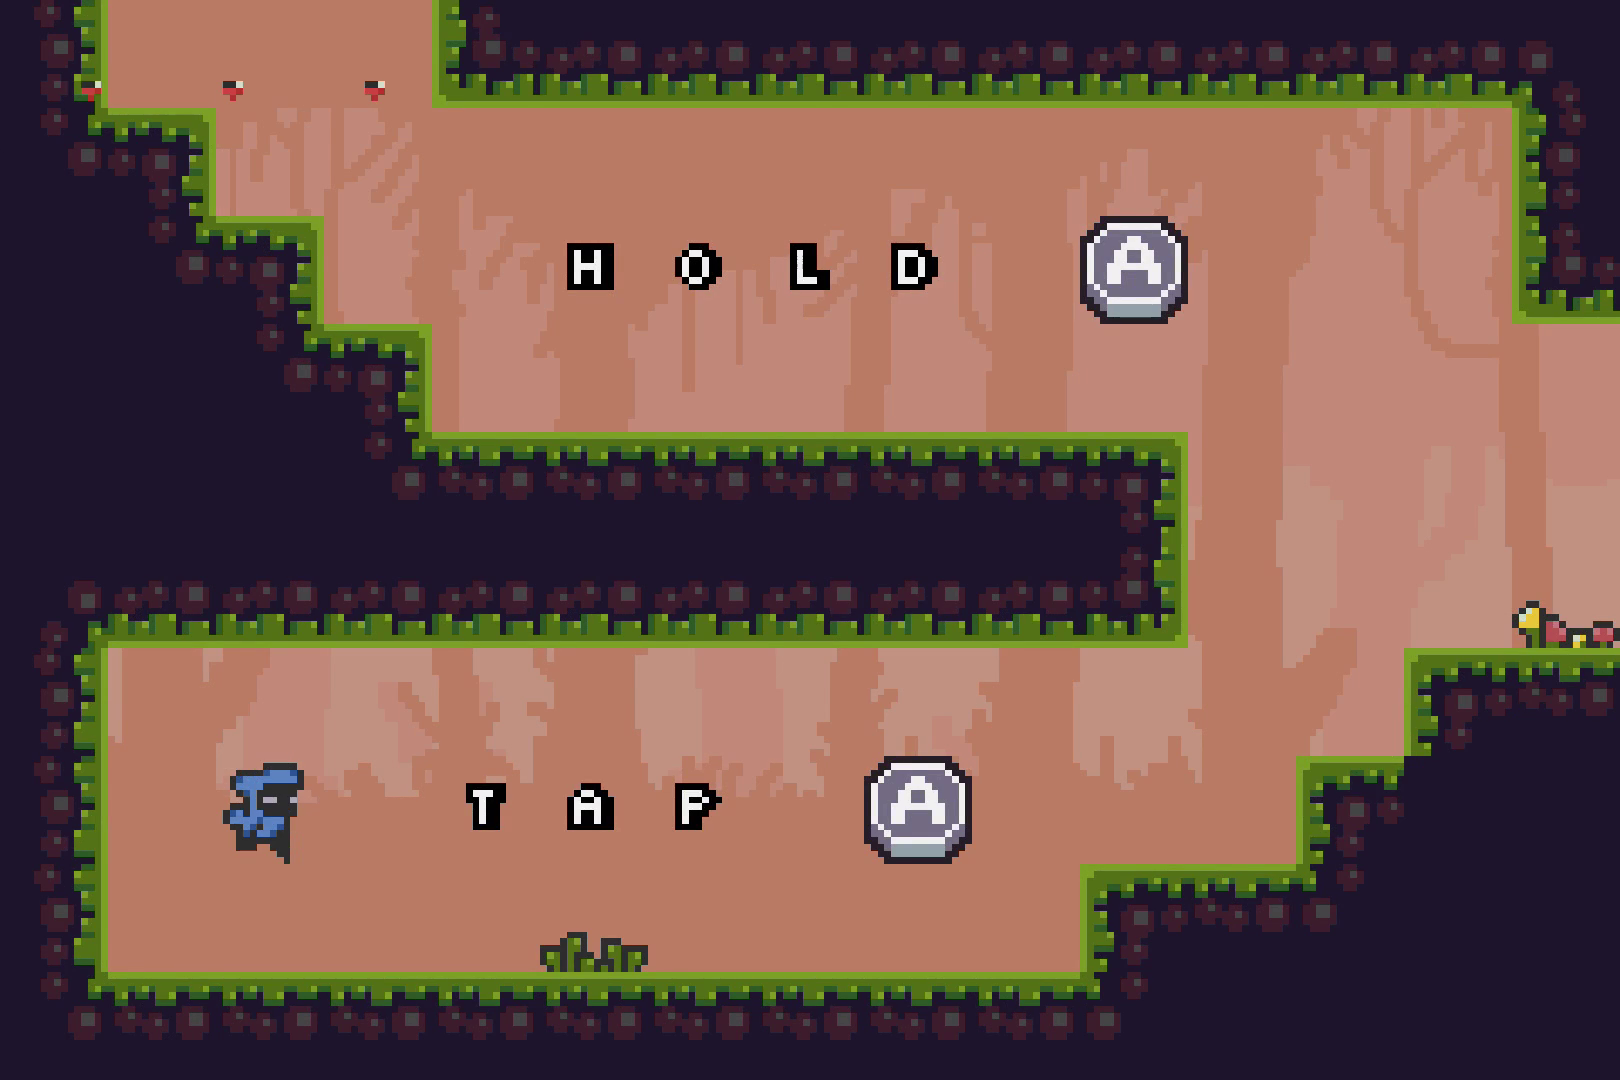
\includegraphics[width=\textwidth]{capitulos/capitulo6/heart_small.png}
		\label{fig:heart_small}
		\caption{Inicio de la animación.}
	\end{subfigure}
	\hfill
	\begin{subfigure}[b]{0.45\textwidth}
		\centering
		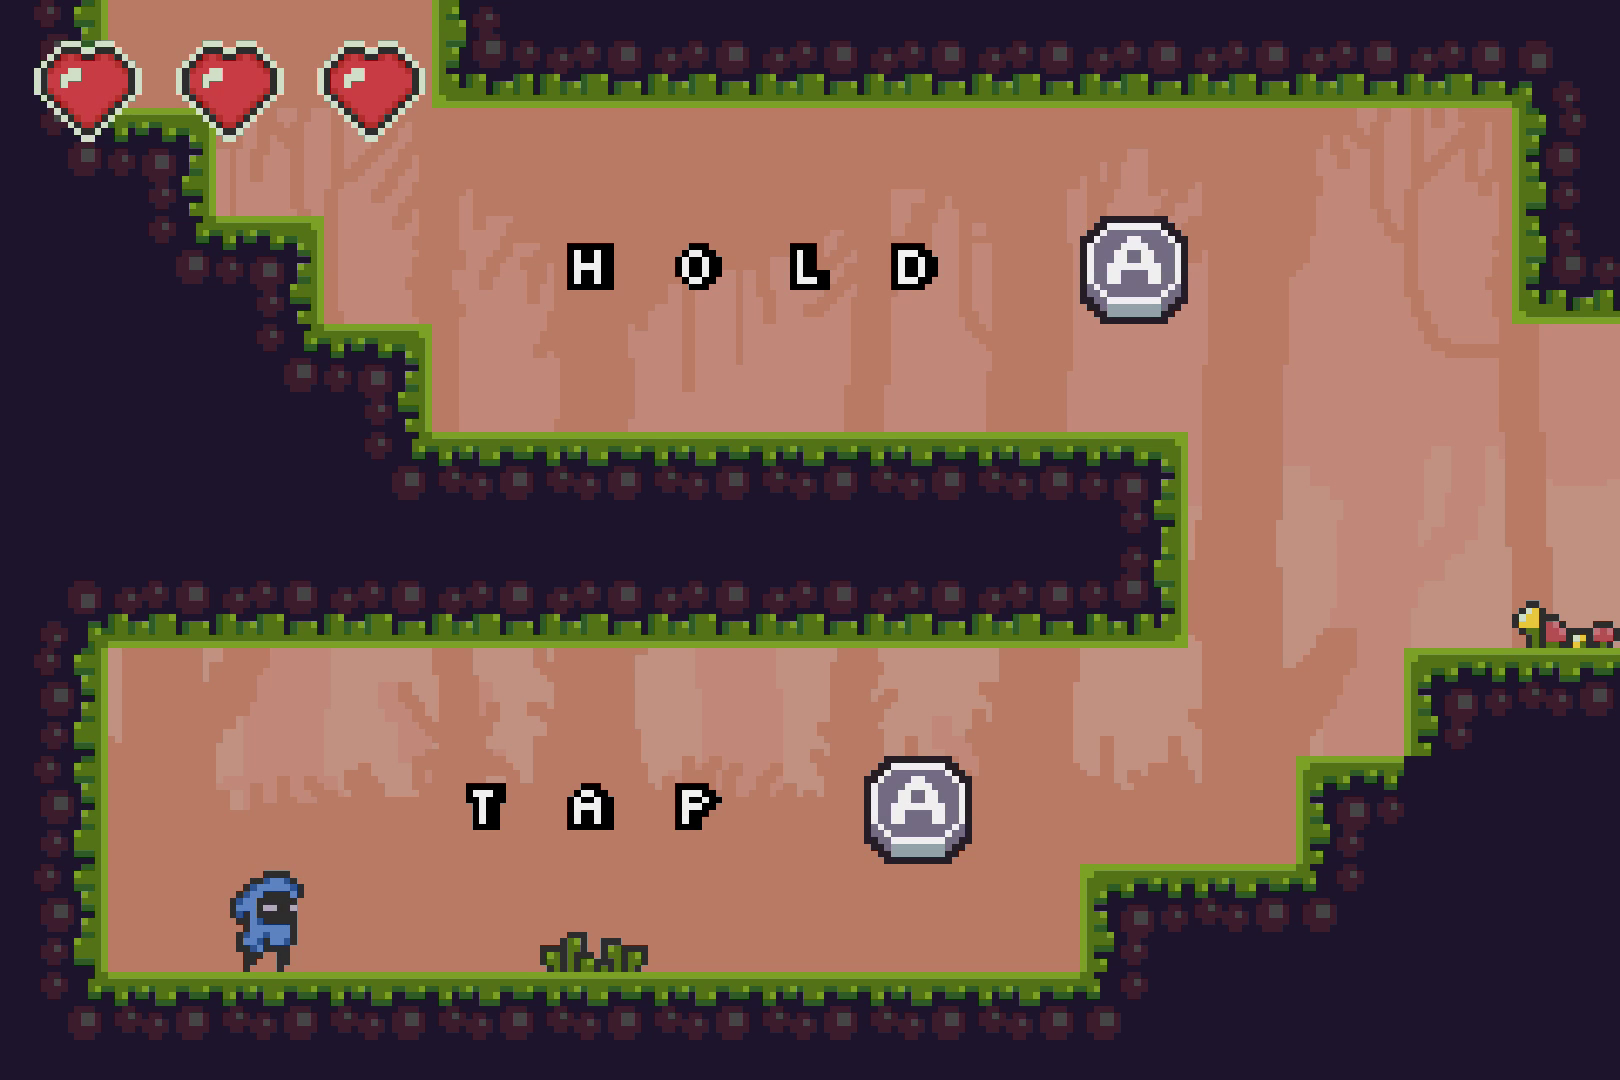
\includegraphics[width=\textwidth]{capitulos/capitulo6/heart_big.png}
		\label{fig:heart_big}
		\caption{Fin de la animación.}
	\end{subfigure}
	\caption{Tres corazones indicando la vida del jugador.}
	\label{fig:heart}
\end{figure}
\FloatBarrier{}


\section{Evaluación del juego en el hardware original}
En esta sección se mostrará el procedimiento a seguir para poder probar el juego en el hardware original. Para ello se hará uso de la tarjeta \textit{Supercard} adquirida junto con el software necesario para cargar el juego en la tarjeta. En el repositorio se incluirá una copia del software dado que no se puede asegurar su disponibilidad en los servidores utilizados por el fabricante para alojarlo.

Con el código compilado, ejecutando el comando ``make'' sobre el directorio raíz del proyecto, se ejecuta el programa ``Super Card'' (véase la Figura~\ref{fig:supercard_software}). Una vez abierto, en la ventana de opciones se seleccionará la tarjeta microSD que se introducirá en el cartucho. Seguidamente, en la ventana principal se seleccionará el juego para procesarlo y guardarlo en la tarjeta.

Seguidamente, se desconecta la tarjeta microSD y se introduce en el cartucho ``Supercard''. Al iniciar la consola, se mostrará un menú con la lista de todos los juegos instalados en la tarjeta. Para abrir el juego, basta con seleccionarlo con el pad direccional y el botón ``A''. En la Figura~\ref{fig:running} se puede observar  el juego ejecutándose en hardware de forma nativa.

\begin{figure}[h]
	\centering
	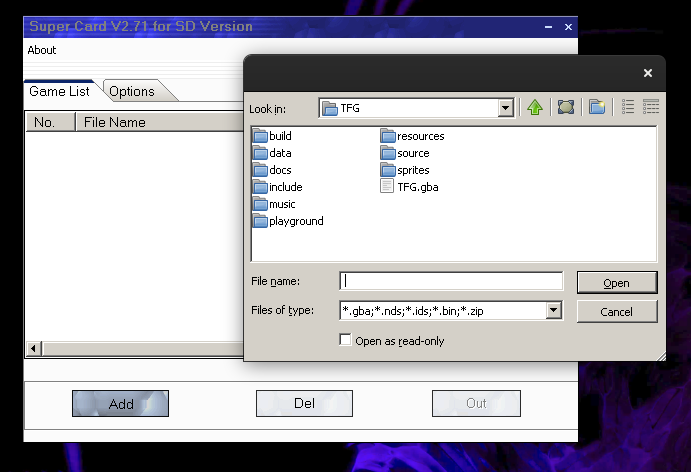
\includegraphics[width=.6\textwidth]{capitulos/capitulo6/supercard.png}
	\caption{Software para meter juegos en el cartucho.}\label{fig:supercard_software}
\end{figure}
\FloatBarrier{}

\begin{figure}[h]
	\centering
	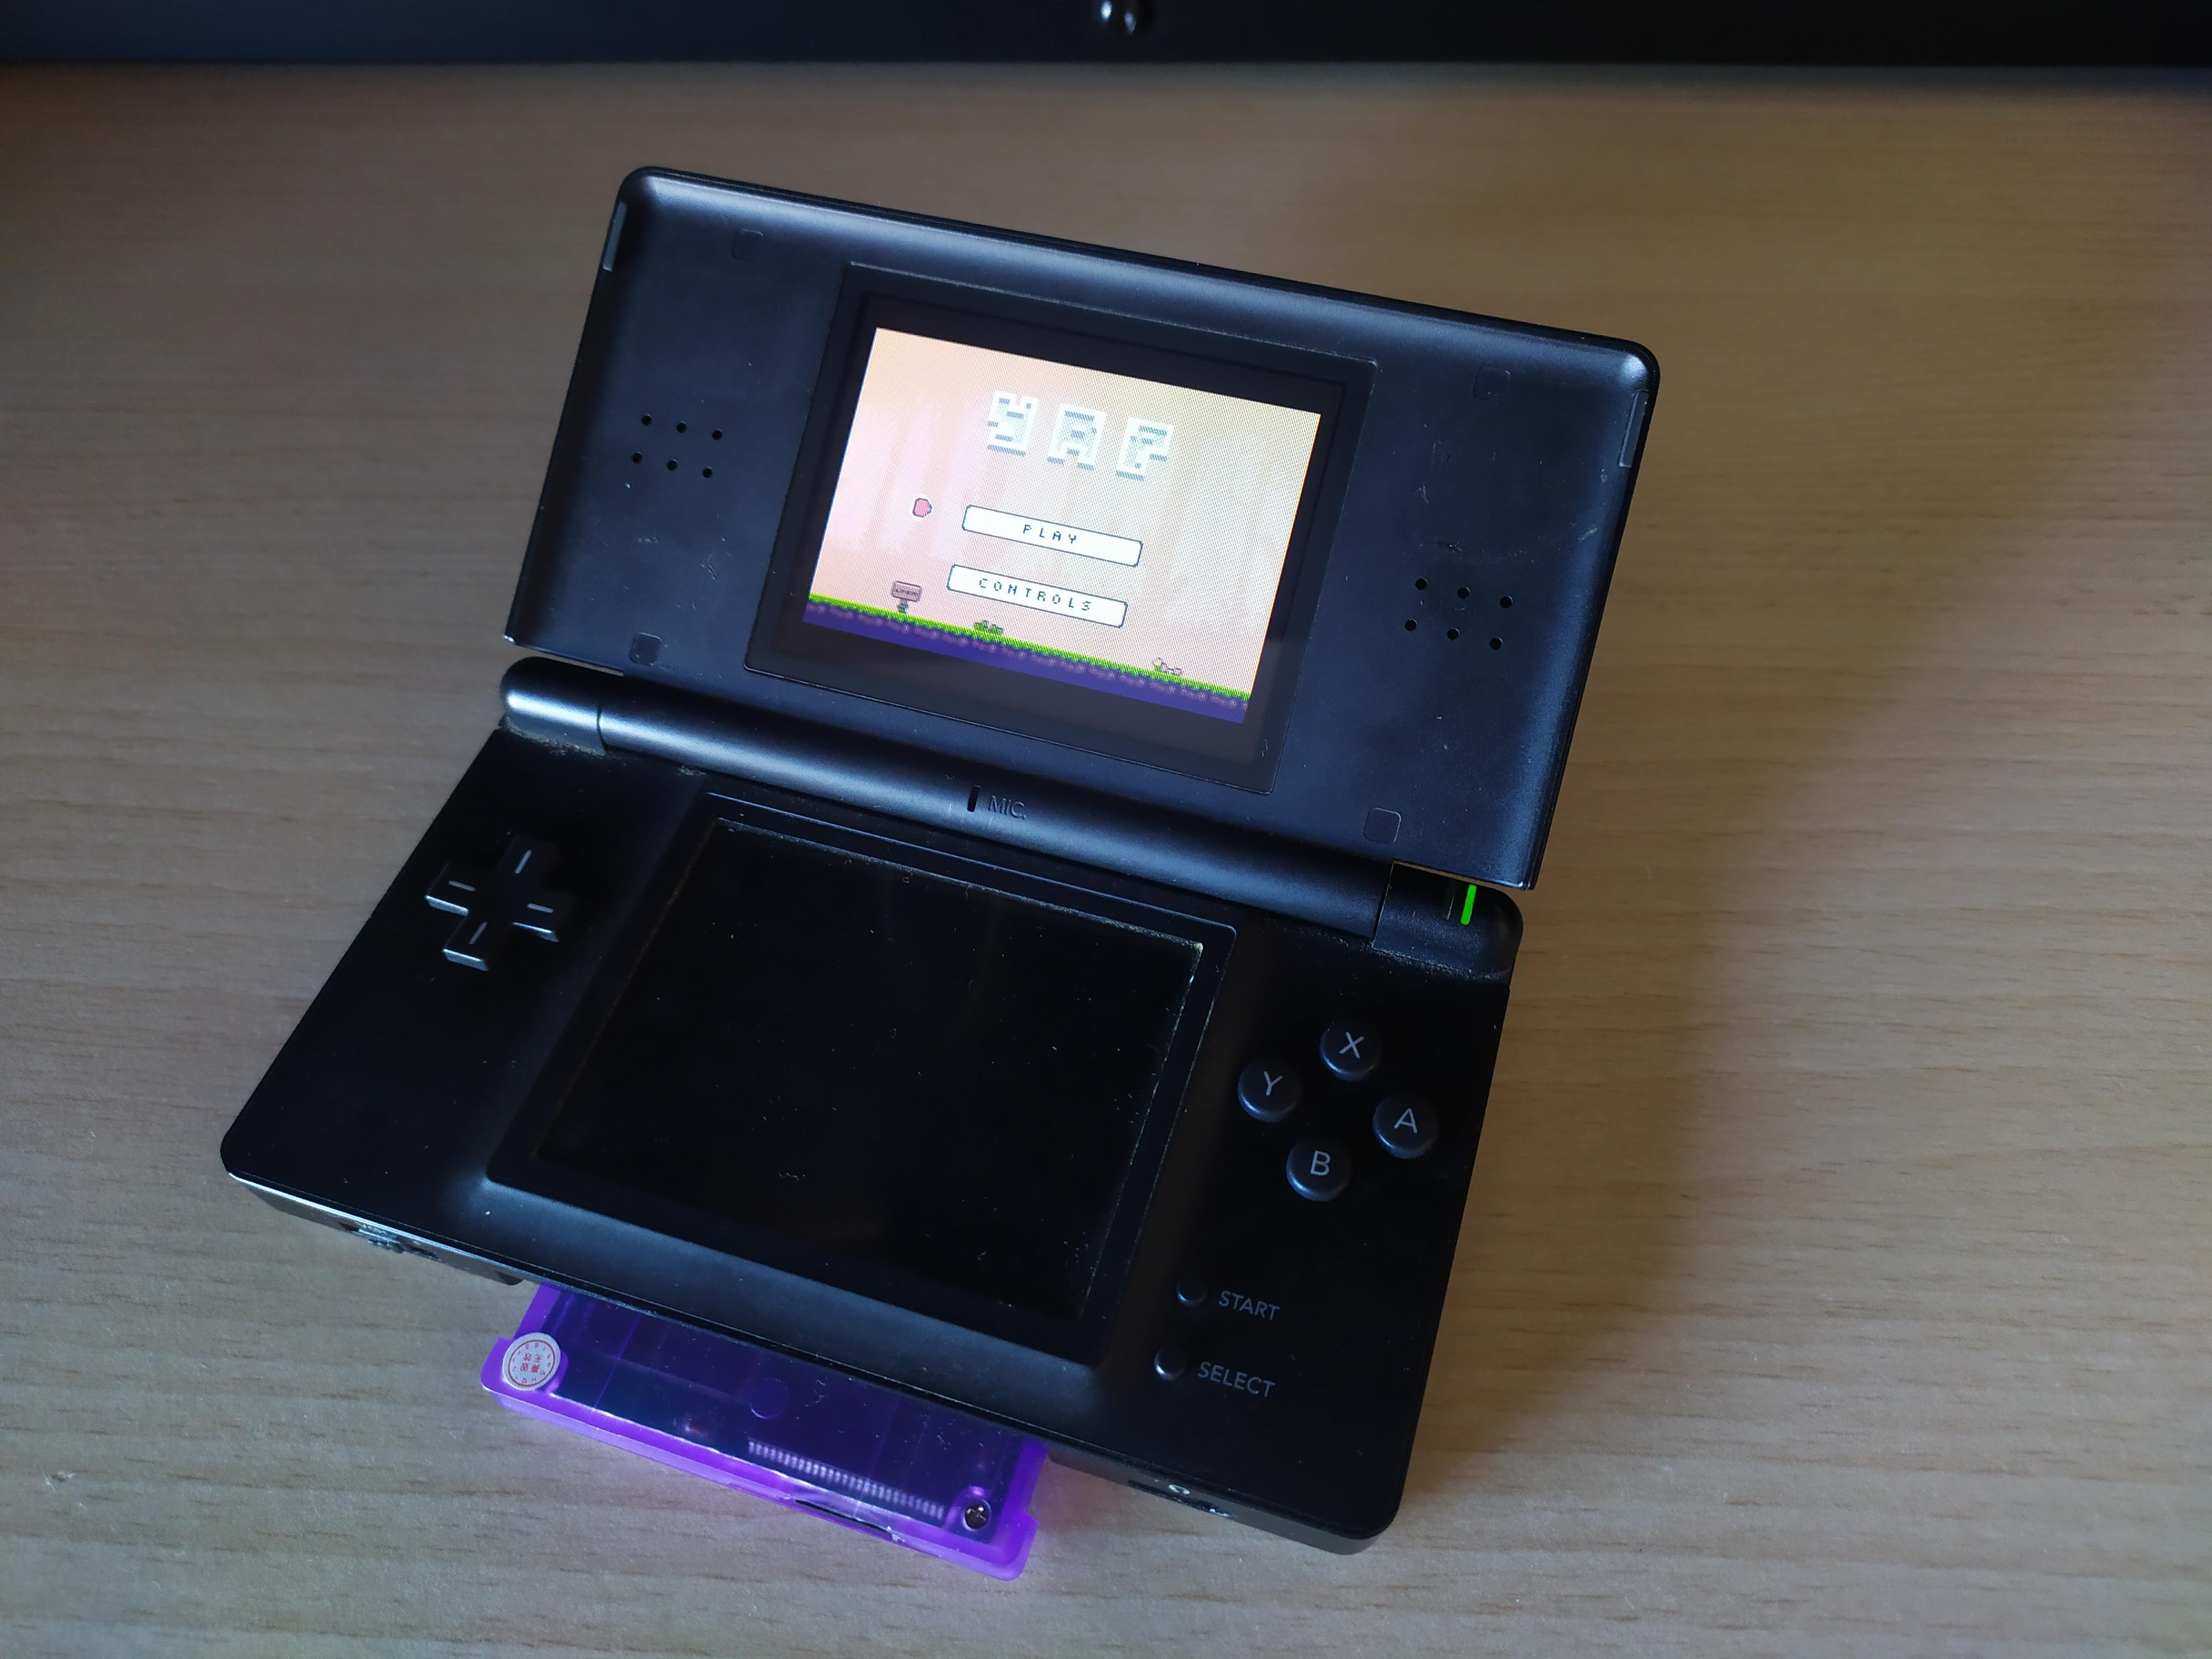
\includegraphics[width=.8\textwidth]{capitulos/capitulo6/running.jpeg}
	\caption{El juego se ejecuta en la Nintendo DS.}\label{fig:running}
\end{figure}
\FloatBarrier{}
